% Created by tikzDevice version 0.6.1 on 2016-06-13 09:43:06
% !TEX encoding = UTF-8 Unicode
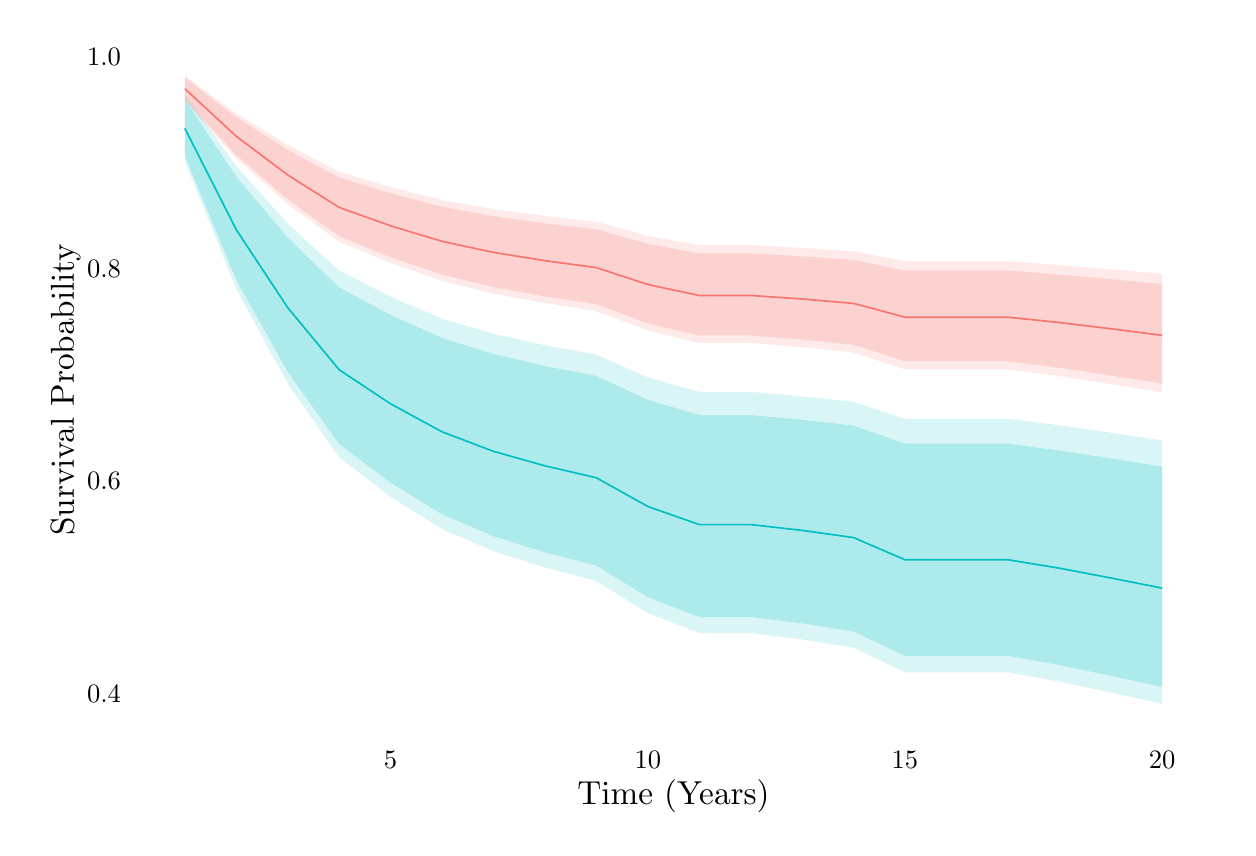
\begin{tikzpicture}[x=1pt,y=1pt]
\definecolor[named]{drawColor}{rgb}{0.00,0.00,0.00}
\definecolor[named]{fillColor}{rgb}{1.00,1.00,1.00}
\fill[color=fillColor,] (0,0) rectangle (433.62,289.08);
\begin{scope}
\path[clip] (  0.00,  0.00) rectangle (433.62,289.08);
\end{scope}
\begin{scope}
\path[clip] (  0.00,  0.00) rectangle (433.62,289.08);
\end{scope}
\begin{scope}
\path[clip] (  0.00,  0.00) rectangle (433.62,289.08);
\end{scope}
\begin{scope}
\path[clip] (  0.00,  0.00) rectangle (433.62,289.08);
\end{scope}
\begin{scope}
\path[clip] (  0.00,  0.00) rectangle (433.62,289.08);
\end{scope}
\begin{scope}
\path[clip] (  0.00,  0.00) rectangle (433.62,289.08);
\end{scope}
\begin{scope}
\path[clip] (  0.00,  0.00) rectangle (433.62,289.08);
\end{scope}
\begin{scope}
\path[clip] (  0.00,  0.00) rectangle (433.62,289.08);
\end{scope}
\begin{scope}
\path[clip] (  0.00,  0.00) rectangle (433.62,289.08);
\end{scope}
\begin{scope}
\path[clip] (  0.00,  0.00) rectangle (433.62,289.08);
\definecolor[named]{drawColor}{rgb}{1.00,1.00,1.00}
\definecolor[named]{fillColor}{rgb}{1.00,1.00,1.00}

\draw[color=drawColor,line width= 0.6pt,line cap=round,line join=round,fill=fillColor,] (  0.00,  0.00) rectangle (433.62,289.08);
\end{scope}
\begin{scope}
\path[clip] (  0.00,  0.00) rectangle (433.62,289.08);
\end{scope}
\begin{scope}
\path[clip] (  0.00,  0.00) rectangle (433.62,289.08);
\end{scope}
\begin{scope}
\path[clip] (  0.00,  0.00) rectangle (433.62,289.08);
\end{scope}
\begin{scope}
\path[clip] ( 39.13, 33.48) rectangle (427.62,283.08);
\definecolor[named]{fillColor}{rgb}{1.00,1.00,1.00}

\draw[fill=fillColor,draw opacity=0.00,] ( 39.13, 33.48) rectangle (427.62,283.08);
\definecolor[named]{drawColor}{rgb}{0.97,0.46,0.43}
\definecolor[named]{fillColor}{rgb}{0.97,0.46,0.43}

\draw[color=drawColor,line width= 0.6pt,line join=round,] ( 56.79,267.03) --
	( 75.38,249.82) --
	( 93.96,235.84) --
	(112.55,224.12) --
	(131.14,217.47) --
	(149.73,211.87) --
	(168.32,207.88) --
	(186.90,204.88) --
	(205.49,202.38) --
	(224.08,196.26) --
	(242.67,192.31) --
	(261.26,192.31) --
	(279.84,191.04) --
	(298.43,189.44) --
	(317.02,184.46) --
	(335.61,184.46) --
	(354.20,184.46) --
	(372.79,182.53) --
	(391.37,180.28) --
	(409.96,177.90);
\definecolor[named]{drawColor}{rgb}{0.00,0.75,0.77}
\definecolor[named]{fillColor}{rgb}{0.00,0.75,0.77}

\draw[color=drawColor,line width= 0.6pt,line join=round,] ( 56.79,252.70) --
	( 75.38,216.07) --
	( 93.96,187.93) --
	(112.55,165.46) --
	(131.14,153.17) --
	(149.73,143.05) --
	(168.32,135.99) --
	(186.90,130.76) --
	(205.49,126.45) --
	(224.08,116.07) --
	(242.67,109.52) --
	(261.26,109.52) --
	(279.84,107.43) --
	(298.43,104.82) --
	(317.02, 96.81) --
	(335.61, 96.81) --
	(354.20, 96.81) --
	(372.79, 93.77) --
	(391.37, 90.23) --
	(409.96, 86.55);
\definecolor[named]{fillColor}{rgb}{0.97,0.46,0.43}

\draw[fill=fillColor,fill opacity=0.15,draw opacity=0.00,] ( 56.79,271.73) --
	( 75.38,258.04) --
	( 93.96,246.68) --
	(112.55,236.99) --
	(131.14,231.47) --
	(149.73,226.81) --
	(168.32,223.50) --
	(186.90,221.00) --
	(205.49,218.91) --
	(224.08,213.81) --
	(242.67,210.51) --
	(261.26,210.51) --
	(279.84,209.50) --
	(298.43,208.29) --
	(317.02,204.64) --
	(335.61,204.64) --
	(354.20,204.64) --
	(372.79,203.30) --
	(391.37,201.75) --
	(409.96,200.13) --
	(409.96,157.30) --
	(391.37,160.31) --
	(372.79,163.17) --
	(354.20,165.60) --
	(335.61,165.60) --
	(317.02,165.60) --
	(298.43,171.72) --
	(279.84,173.67) --
	(261.26,175.17) --
	(242.67,175.17) --
	(224.08,179.68) --
	(205.49,186.70) --
	(186.90,189.57) --
	(168.32,193.00) --
	(149.73,197.60) --
	(131.14,204.05) --
	(112.55,211.73) --
	( 93.96,225.33) --
	( 75.38,241.79) --
	( 56.79,262.39) --
	cycle;
\definecolor[named]{fillColor}{rgb}{0.00,0.75,0.77}

\draw[fill=fillColor,fill opacity=0.15,draw opacity=0.00,] ( 56.79,264.97) --
	( 75.38,239.05) --
	( 93.96,218.24) --
	(112.55,201.29) --
	(131.14,191.83) --
	(149.73,183.97) --
	(168.32,178.44) --
	(186.90,174.34) --
	(205.49,170.93) --
	(224.08,162.68) --
	(242.67,157.49) --
	(261.26,157.49) --
	(279.84,155.86) --
	(298.43,153.90) --
	(317.02,147.76) --
	(335.61,147.76) --
	(354.20,147.76) --
	(372.79,145.42) --
	(391.37,142.73) --
	(409.96,139.93) --
	(409.96, 44.82) --
	(391.37, 48.87) --
	(372.79, 52.78) --
	(354.20, 56.16) --
	(335.61, 56.16) --
	(317.02, 56.16) --
	(298.43, 65.06) --
	(279.84, 68.01) --
	(261.26, 70.33) --
	(242.67, 70.33) --
	(224.08, 77.58) --
	(205.49, 89.15) --
	(186.90, 93.99) --
	(168.32, 99.91) --
	(149.73,107.93) --
	(131.14,119.55) --
	(112.55,133.84) --
	( 93.96,160.47) --
	( 75.38,194.63) --
	( 56.79,240.83) --
	cycle;
\definecolor[named]{fillColor}{rgb}{0.97,0.46,0.43}

\draw[fill=fillColor,fill opacity=0.20,draw opacity=0.00,] ( 56.79,270.97) --
	( 75.38,256.71) --
	( 93.96,244.91) --
	(112.55,234.89) --
	(131.14,229.18) --
	(149.73,224.36) --
	(168.32,220.94) --
	(186.90,218.35) --
	(205.49,216.20) --
	(224.08,210.92) --
	(242.67,207.51) --
	(261.26,207.51) --
	(279.84,206.46) --
	(298.43,205.18) --
	(317.02,201.30) --
	(335.61,201.30) --
	(354.20,201.30) --
	(372.79,199.86) --
	(391.37,198.19) --
	(409.96,196.44) --
	(409.96,160.51) --
	(391.37,163.42) --
	(372.79,166.19) --
	(354.20,168.54) --
	(335.61,168.54) --
	(317.02,168.54) --
	(298.43,174.49) --
	(279.84,176.39) --
	(261.26,177.86) --
	(242.67,177.86) --
	(224.08,182.28) --
	(205.49,189.17) --
	(186.90,191.98) --
	(168.32,195.34) --
	(149.73,199.85) --
	(131.14,206.17) --
	(112.55,213.69) --
	( 93.96,227.00) --
	( 75.38,243.07) --
	( 56.79,263.13) --
	cycle;
\definecolor[named]{fillColor}{rgb}{0.00,0.75,0.77}

\draw[fill=fillColor,fill opacity=0.20,draw opacity=0.00,] ( 56.79,262.97) --
	( 75.38,235.25) --
	( 93.96,213.16) --
	(112.55,195.22) --
	(131.14,185.24) --
	(149.73,176.96) --
	(168.32,171.14) --
	(186.90,166.83) --
	(205.49,163.24) --
	(224.08,154.57) --
	(242.67,149.11) --
	(261.26,149.11) --
	(279.84,147.39) --
	(298.43,145.29) --
	(317.02,138.77) --
	(335.61,138.77) --
	(354.20,138.77) --
	(372.79,136.29) --
	(391.37,133.42) --
	(409.96,130.44) --
	(409.96, 50.86) --
	(391.37, 54.88) --
	(372.79, 58.75) --
	(354.20, 62.09) --
	(335.61, 62.09) --
	(317.02, 62.09) --
	(298.43, 70.90) --
	(279.84, 73.82) --
	(261.26, 76.11) --
	(242.67, 76.11) --
	(224.08, 83.28) --
	(205.49, 94.71) --
	(186.90, 99.49) --
	(168.32,105.32) --
	(149.73,113.22) --
	(131.14,124.64) --
	(112.55,138.66) --
	( 93.96,164.70) --
	( 75.38,197.97) --
	( 56.79,242.71) --
	cycle;
\end{scope}
\begin{scope}
\path[clip] (  0.00,  0.00) rectangle (433.62,289.08);
\end{scope}
\begin{scope}
\path[clip] (  0.00,  0.00) rectangle (433.62,289.08);
\end{scope}
\begin{scope}
\path[clip] (  0.00,  0.00) rectangle (433.62,289.08);
\end{scope}
\begin{scope}
\path[clip] (  0.00,  0.00) rectangle (433.62,289.08);
\end{scope}
\begin{scope}
\path[clip] (  0.00,  0.00) rectangle (433.62,289.08);
\end{scope}
\begin{scope}
\path[clip] (  0.00,  0.00) rectangle (433.62,289.08);
\definecolor[named]{drawColor}{rgb}{0.00,0.00,0.00}

\node[color=drawColor,anchor=base east,inner sep=0pt, outer sep=0pt, scale=  0.96] at ( 33.73, 45.38) {0.4%
};

\node[color=drawColor,anchor=base east,inner sep=0pt, outer sep=0pt, scale=  0.96] at ( 33.73,122.03) {0.6%
};

\node[color=drawColor,anchor=base east,inner sep=0pt, outer sep=0pt, scale=  0.96] at ( 33.73,198.67) {0.8%
};

\node[color=drawColor,anchor=base east,inner sep=0pt, outer sep=0pt, scale=  0.96] at ( 33.73,275.31) {1.0%
};
\end{scope}
\begin{scope}
\path[clip] (  0.00,  0.00) rectangle (433.62,289.08);
\end{scope}
\begin{scope}
\path[clip] (  0.00,  0.00) rectangle (433.62,289.08);
\end{scope}
\begin{scope}
\path[clip] (  0.00,  0.00) rectangle (433.62,289.08);
\end{scope}
\begin{scope}
\path[clip] (  0.00,  0.00) rectangle (433.62,289.08);
\end{scope}
\begin{scope}
\path[clip] (  0.00,  0.00) rectangle (433.62,289.08);
\end{scope}
\begin{scope}
\path[clip] (  0.00,  0.00) rectangle (433.62,289.08);
\end{scope}
\begin{scope}
\path[clip] (  0.00,  0.00) rectangle (433.62,289.08);
\end{scope}
\begin{scope}
\path[clip] (  0.00,  0.00) rectangle (433.62,289.08);
\end{scope}
\begin{scope}
\path[clip] (  0.00,  0.00) rectangle (433.62,289.08);
\end{scope}
\begin{scope}
\path[clip] (  0.00,  0.00) rectangle (433.62,289.08);
\end{scope}
\begin{scope}
\path[clip] (  0.00,  0.00) rectangle (433.62,289.08);
\end{scope}
\begin{scope}
\path[clip] (  0.00,  0.00) rectangle (433.62,289.08);
\definecolor[named]{drawColor}{rgb}{0.00,0.00,0.00}

\node[color=drawColor,anchor=base,inner sep=0pt, outer sep=0pt, scale=  0.96] at (131.14, 21.46) {5%
};

\node[color=drawColor,anchor=base,inner sep=0pt, outer sep=0pt, scale=  0.96] at (224.08, 21.46) {10%
};

\node[color=drawColor,anchor=base,inner sep=0pt, outer sep=0pt, scale=  0.96] at (317.02, 21.46) {15%
};

\node[color=drawColor,anchor=base,inner sep=0pt, outer sep=0pt, scale=  0.96] at (409.96, 21.46) {20%
};
\end{scope}
\begin{scope}
\path[clip] (  0.00,  0.00) rectangle (433.62,289.08);
\end{scope}
\begin{scope}
\path[clip] (  0.00,  0.00) rectangle (433.62,289.08);
\end{scope}
\begin{scope}
\path[clip] (  0.00,  0.00) rectangle (433.62,289.08);
\end{scope}
\begin{scope}
\path[clip] (  0.00,  0.00) rectangle (433.62,289.08);
\definecolor[named]{drawColor}{rgb}{0.00,0.00,0.00}

\node[color=drawColor,anchor=base,inner sep=0pt, outer sep=0pt, scale=  1.20] at (233.37,  8.40) {Time (Years)%
};
\end{scope}
\begin{scope}
\path[clip] (  0.00,  0.00) rectangle (433.62,289.08);
\end{scope}
\begin{scope}
\path[clip] (  0.00,  0.00) rectangle (433.62,289.08);
\definecolor[named]{drawColor}{rgb}{0.00,0.00,0.00}

\node[rotate= 90.00,color=drawColor,anchor=base,inner sep=0pt, outer sep=0pt, scale=  1.20] at ( 16.66,158.28) {Survival Probability%
};
\end{scope}
\begin{scope}
\path[clip] (  0.00,  0.00) rectangle (433.62,289.08);
\end{scope}
\begin{scope}
\path[clip] (  0.00,  0.00) rectangle (433.62,289.08);
\end{scope}
\begin{scope}
\path[clip] (  0.00,  0.00) rectangle (433.62,289.08);
\end{scope}
\begin{scope}
\path[clip] (  0.00,  0.00) rectangle (433.62,289.08);
\end{scope}
\end{tikzpicture}
